\documentclass[10pt]{article}
\usepackage[pdftex]{graphicx, color}
\usepackage{listings}
\usepackage{amsmath}

\usepackage{tikz}
\usetikzlibrary{automata,positioning}

\headheight 8pt \headsep 20pt \footskip 30pt
\textheight 9in \textwidth 6.5in
\oddsidemargin 0in \evensidemargin 0in
\topmargin -.35in

\lstset{basicstyle=\small\ttfamily,breaklines=true}
\newcommand {\pts}[1]{{\bf #1 pts}}
\newcommand{\ttmath}[1]{$\mathtt{#1}$}
\newcommand{\ossimple}[6]{#1,#2,#3\vdash #4 : #5,#6}
\newcommand{\osrule}[8]{\frac{#7}{\ossimple{#1}{#2}{#3}{#4}{#5}{#6}}\eqno
  \mbox{#8}}

\newcommand{\deduct}[3]{\frac{#1}{#2}\eqno\mbox{#3}}


\begin{document}
\begin{center}
\Large CS131 Compilers: Writing Assignment 4\\Due Tuesday, June 12, 2018 at 23:59
\end{center}

\begin{center}
%% Change this:
\LARGE Yuyang Rong - 69850764
\end{center}

This assignment asks you to prepare written answers to questions on
run-time environment, object layout, operational semantics, code generation, register allocation and garbage collection.
Each of the questions has a short answer. You
may discuss this assignment with other students and work on the problems
together. However, your write-up should be your own individual work,
and you should indicate in your submission who you worked with, if applicable.
You should use the Latex template provided at the course web site to write your solution.

\begin{center}
%% Change this:
I worked with: (Name,ID), (Name,ID)...
\end{center}

Example for operational semantics rule in tex:
$$\osrule{so}{S_1} E {\mbox{while }e_1\mbox{ loop } e_2\mbox{ pool}}{void}{S_{2}}
	{\begin{array}{l}
	\ossimple{so}{S_1}{E}{e_1}{Bool(false)}{S_2}\\
	 \end{array}}{[Loop-False]}
$$

\begin{enumerate}

\item (10 pts)
Consider the following Cool classes:

\begin{center}
\begin{minipage}{6cm}
\begin{verbatim}
class A {
    a1 : Int;
    a2 : String;
    m1() : Object { ... };
    m2() : Object { ... };
};

class B inherits A {
    a3 : Int;
    m1() : Object { ... };
    m3() : Object { ... };
};

class C inherits B {
    a4 : Int;
    m2() : Object { ... };
    m3() : Object { ... };
};
\end{verbatim}
\end{minipage}
\end{center}
\begin{enumerate}

\item Draw a diagram that illustrates the layout of objects of type {\tt
A}, {\tt B} and {\tt C}, including their dispatch tables.

\begin{table}[ht]
	\centering
	\caption{Object Layout}
	\begin{tabular}{|c|c|c|c|c|}                         \hline
		Offset & A     & B     & C     & Explanation  \\ \hline
		0      & A tag & B tag & C tag & Class tag    \\ \hline
		4      & 5     & 6     & 7     & Object Size  \\ \hline
		12     & *     & *     & *     & Dispatch Ptr \\ \hline
		16     & a1    & a1    & a1    & Attribute    \\ \hline
		20     & a2    & a2    & a2    & Attribute    \\ \hline
		24     & N/A   & a3    & a3    & Attribute    \\ \hline
		28     & N/A   & N/A   & a4    & Attribute    \\ \hline
	\end{tabular}
\end{table}

\begin{table}[ht]
	\centering
	\caption{Dispatch Table}
	\begin{tabular}{|c|c|c|c|}               \hline
		Offset & A      & B      & C      \\ \hline
		0      & A.m1() & B.m1() & B.m1() \\ \hline
		4      & A.m2() & A.m2() & C.m2() \\ \hline
		12     &  N/A   & B.m3() & C.m3() \\ \hline
	\end{tabular}
\end{table}

\item Let {\tt obj} be a variable whose static type is {\tt A}.  Assume
that {\tt obj} is stored in register {\tt \$a0}.  Write MIPS code for the
function invocation {\tt obj.m2()}.  You may use temporary registers
such as {\tt \$t0} if you wish.

\begin{lstlisting}
	lw      $t0,    12($a0)   # Get access to dispatch table.
	lw      $t0,    4($t0) 	  # Get function pointer
	jal     $t0               # This doesn't seem right.
\end{lstlisting}
\item Explain what happens in part (b) if {\tt obj} has dynamic type {\tt
B}.

When {\tt obj} has dynamic type B, the processor will look for B's dispatch table and call the function listed inside, even though they may be the same function that is inherited from A.
\end{enumerate}

\pagebreak

\item (10 pts)
Suppose you wish to add arrays to Cool using the following syntax:

\begin{center}
\begin{tabular}{ll}
\texttt{let a:T[\ttmath{e_1}] in \ttmath{e_2}} &
  Create an array $a$ with size $e_1$ of $T$'s, usable in $e_2$ \\
\texttt{a[\ttmath{e_1}] <- \ttmath{e_2}} &
  Assign $e_2$ to element $e_1$ in $a$ \\
\texttt{a[e]} &
  Get element $e$ of $a$
\end{tabular}
\end{center}

Write the operational semantics for these three syntactic constructs. You
may find it helpful to think of an array of type $T[n]$ as an object with
$n$ attributes of type $T$. \\

\texttt{let a:T[\ttmath{e_1}] in \ttmath{e_2}} \\
$$
\deduct{
	\begin{array}{l}
		\ossimple{so}{S_1}{E}{T[e_1]}{void}{S_2}		 \\
		l_1 = newloc(S_2)								\\
		S_3 = S_2[void / l_1] 							\\
		E' = E[l_1 / a] 								\\
		\ossimple{so}{S_3}{E'}{e_2}{v_2}{S_4} 			\\
	\end{array}
}{
	\ossimple{so}{S_1}{E}{\texttt{let a:T[\ttmath{e_1}] in \ttmath{e_2}}}{v_2}{S_4}\\
}{
	[Let-Array]}
$$

\texttt{a[\ttmath{e_1}] \ttmath{\leftarrow e_2}} \\
$$
\deduct{
	\begin{array}{l}
		\ossimple{so}{S_1}{E}{e_2}{v}{S_2}	\\
		E(a[e_1]) = l_a 					\\
		S = S_1[v/l_a]						\\
	\end{array}
}{
	\ossimple{so}{S_1}{E}{\texttt{a[\ttmath{e_1}] \ttmath{\leftarrow e_2}} } {v}{S} \\
}{
	[Assign-Array]
}
$$
\texttt{a[e]} \\
$$\deduct{
	\begin{array}{l}
		E(a[e]) = l_a 	\\
		S(l_a) = v 		\\
	\end{array}	
}{
	\ossimple{so}{S_1}{E}{\texttt{a[e]}}{v}{S} \\	
}{
	[Reference-Array]
}$$

\pagebreak

\item (10 pts)
The operational semantics for Cool's {\tt while} expression show that
result of evaluating such an expression is always {\tt void}.  (See page
28 of the Cool manual.)

However, we could have used the following alternative semantics:

\begin{itemize}

\item If the loop body executes at least once, the result of the {\tt
while} expression is the result from the last iteration of the loop body.

\item If the loop body never executes (i.e., the condition is false the
first time it is evaluated), then the result of the {\tt while} expression
is {\tt void}.

\end{itemize}

For example, consider the following expression:

\begin{center}
{\tt while (x < 10) loop x <- x+1 pool}
\end{center}

The result of this expression would be 10 if {\tt x} $<$ 10 or {\tt void}
if {\tt x} $\geq$ 10.

Write new operational rules for the {\tt while} construct that formalize
these alternative semantics.


\item (10 pts) Consider the following MIPS assembly code program.  Using the
stack-machine based code generation rules from lecture, what source program produces this
code?
\begin{verbatim}
f_entry:
        move  $fp $sp
        sw    $ra 0($sp)
        addiu $sp $sp -4
        lw    $a0 4($fp)
        sw    $a0 0($sp)
        addiu $sp $sp -4
        li    $a0 0
        lw    $t1 4($sp)
        addiu $sp $sp 4
        beq   $a0 $t1 true_branch
false_branch:
        lw    $a0 4($fp)
        sw    $a0 0($sp)
        addiu $sp $sp -4
        sw    $fp 0($sp)
        addiu $sp $sp -4
        lw    $a0 4($fp)
        sw    $a0 0($sp)
        addiu $sp $sp -4
        li    $a0 1
        lw    $t1 4($sp)
        sub   $a0 $t1 $a0
        addiu $sp $sp 4
        sw    $a0 0($sp)
        addiu $sp $sp -4
        jal   f_entry
        lw    $t1 4($sp)
        add   $a0 $a0 $t1
        addiu $sp $sp 4
        b     end_if
true_branch:
        li    $a0 0
end_if:
        lw    $ra 4($sp)
        addiu $sp $sp 12
        lw    $fp 0($sp)
        jr    $ra
\end{verbatim}

\begin{lstlisting}
void fib(const unsigned int a){
    if (a == 0){
        return 0;
    } else {
        int temp = a - 1;
        return fib(temp) + temp;
    }
}
\end{lstlisting}

\pagebreak

\item (10 pts) Give a recursive definition of the cgen function for the following new construct.
\begin{eqnarray*}
\tt{for}\;\; i = e_1 \;\;to\;\; e_2 \;\;\tt{by}\;\; e_3 \;\;\tt{do }\;\; e_4
\end{eqnarray*}

Assume that the subexpressions $e_1, e_2, e_3$ and $e_4$ are
integer-valued. A ``for loop'' expression is evaluated according to
the following rules. The first three subexpressions are evaluated once
at the start of the loop in the order $e_1$, $e_2$, and then $e_3$.
The subexpression $e_4$ is evaluated once per iteration of the loop.
The index variable $i$ is initialized to the value of $e_1$.
The loop bound is the value of $e_2$ and $i$ is incremented by the
value of $e_3$ after each iteration. The loop terminates before
executing an iteration where the value of $i$ is greater than the
loop bound. The value returned by the ``for loop'' expression is the value of the
expression $e_4$ in the last iteration. If the loop does not execute
at all, then the value returned is the integer $0$.

Following is a more formal semantics of the for expression in terms of the Cool
expressions.
\begin{tabbing}
  \hspace*{3mm} \= let t: Int $\leftarrow$ $e_1$ in \\
  \> let bound:Int  $\leftarrow$ $e_2$ in \\
  \> let incr:Int  $\leftarrow$ $e_3$ in \\
  \> let result:Int  $\leftarrow$ $0$ in \\
  \> let \= i:Int $\leftarrow$ $t$ in   \\
   \>  \> while \= ($i$ $\leq$ bound) loop \{ \\
     \>\>\>   result $\leftarrow$ $e_4$; \\
\> \> \> $i$ $\leftarrow$ $i$ + incr; \\
     \> \> \} pool; \\
     \> \> result  \\
\end{tabbing}

Note that the expressions $e_1$, $e_2$ and $e_3$ are evaluated ONLY once before the start of the loop.
Also note that any occurences of variable $i$ in $e_1$, $e_2$ and
$e_3$ refer to the value of $i$
just before the for loop.
Any occurrence of variable $i$ in expression $e_4$ refers to the loop index variable $i$.


\begin{equation}\begin{aligned}
	  & \text{cgen}(\tt{for}\;\; i = e_1 \;\;to\;\; e_2 \;\;\tt{by}\;\; e_3 \;\;\tt{do }\;\; e_4) \\
	= & \text{cgen} (e_1) 		\\
	  & \$a1 \leftarrow \$a0	\\
	  & \text{cgen} (e_2) 		\\
	  & \$a2 \leftarrow \$a0	\\
	  & \text{cgen} (e_3) 		\\
	  & \$a3 \leftarrow \$a0	\\
	  & \text{push } \$a1 		\\
	\text{Loop: } \\
	  & \$t0 \leftarrow top 	\\
	  & \text{bge } \$a2 \text{ } \$t0 \text{ true\_branch} \\
	\text{false\_branch: }  \\
	  & \text{b EndLoop}		\\
	\text{true\_branch: }	\\
	  & \text{cgen} (e_4) 		\\
	  & \text{pop} 				\\
	  & \text{addiu } \$t0, \$t0, \$a3 	\\
	  & \text{push } \$t0 		\\
	  & \text{b Loop} 			\\
	\text{EndLoop: } 		\\
\end{aligned}\end{equation}

\pagebreak

\item (2*10=20 pts) Consider the following program:

\begin{verbatim}
L0: e := 0
    b := 1;
    d := 2;
L1: a := b+2
    c := d+5
    e := e + c
    f := a * a
    if f < c goto L3
L2: e := e + f
    goto L4
L3: e := e + 2
L4: d := d + 4
    b := b - 4
    if b != d goto L1
L5:
\end{verbatim}

This program uses six temporaries \texttt{a}-\texttt{f}.  Assume that
our machine has only 4 available registers \texttt{\$r0},
\texttt{\$r1}, \texttt{\$r2}, and \texttt{\$r3}
and that only
\texttt{e} is live on exit from this program.

\begin{enumerate}
\item Draw the register interference graph.  (Computing the sets of
live variables at every program point may be helpful for this step.)

\item Use the graph coloring heuristics discussed in lecture to assign
  each temporary to a register on a machine that has $4$ registers.
Rewrite the program replacing temporaries by registers and including whatever
spill code is necessary.  Use the pseudo-instructions \texttt{load x}
and \texttt{store x} to load and spill the value of \texttt{x} from
memory.
\end{enumerate}

We will start by compute the set of live vars first:

\begin{lstlisting}[tabsize=4]
L0: e := 0 				# {e}		 
    b := 1;				# {b, d}		
    d := 2;				# {b, d, e}		
L1: a := b+2			# {a, b, d, e}		
    c := d+5			# {a, b, c, d, e}		
    e := e + c 			# {a, b, c, d, e}		
    f := a * a 			# {b, c, d, e, f}		
    if f < c 			# {b, d, e, f}		
    	goto L3			# {b, d, e}		
L2: e := e + f 			# {b, d, e}		
    goto L4				# 
L3: e := e + 2			# {b, d, e}		
L4: d := d + 4			# {b, d, e}		
    b := b - 4			# {b, d, e}		
    if b != d 			# {b, d, e} 
    	goto L1	# {}	# {b, d, e}
L5:						# {e}
\end{lstlisting}

\begin{center}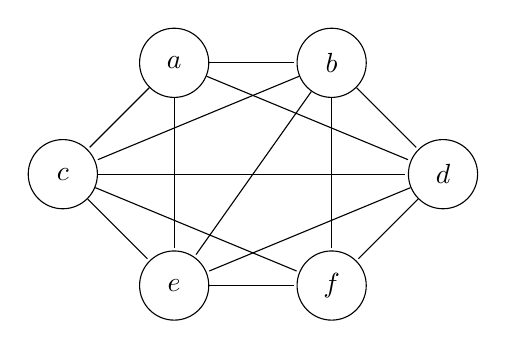
\begin{tikzpicture}[shorten >=1pt,node distance=2cm,on grid,auto]
	\node[state] 			(c) 						{$c$};
	\node[state] 			(a) 	[above right=of c]	{$a$};
	\node[state]			(e) 	[below right=of c] 	{$e$};
	\node[state] 			(b) 	[	   right=of a] 	{$b$};
	\node[state] 			(d) 	[below right=of b] 	{$d$};
	\node[state] 			(f) 	[	   right=of e]	{$f$};
	\path[-]
	(a) 	edge	node	{} 		(b)
			edge	node	{} 		(c)
			edge	node	{} 		(d)
			edge	node	{} 		(e)
	(b) 	edge	node	{} 		(c)
			edge	node	{} 		(d)
			edge	node	{} 		(e)
			edge	node	{} 		(f)
	(c)		edge	node	{} 		(d)
			edge	node	{} 		(e)
			edge	node	{} 		(f)
	(d) 	edge	node	{} 		(e)
			edge	node	{} 		(f)
	(e) 	edge	node	{} 		(f);
\end{tikzpicture}\end{center}


\pagebreak

\item (10*3=30 pts) Consider the following Cool program:

\begin{verbatim}
class C {
  x : C; y : C;
  setx(newx : C) : C { x <- newx };
  sety(newy : C) : C { y <- newy };
  setxy(newx : C, newy :C) : SELFT_TYPE {{ x <- newx; y <- newy; self; }};
};

class Main {
  x:C;
  main() : Object {
    let a : C <- new C, b :C <- new C, c : C<- new C, d : C <- new C,
    e : C <- new C, f :C <- new C, g : C <- new C, h : C <- new C in {
      f.sety(g); a.setxy(e, c); b.setx(f); g.setxy(f,d); c.sety(h); h.setxy(e, a); x <- c;
    }
  };
};
\end{verbatim}
\begin{enumerate}
  \item (10 pts) Draw the heap at the end of execution of the above program, identifying objects by the variable names to which they are bound in the let expression. Assume that the root is the Main object created at the start of the program, and this object is not in the heap (note that Main is pointing to c).
%
  \item (10 pts) For each of the garbage collection algorithms discussed in class (Mark and Sweep, Stop and Copy,
Reference Counting), show the heap after garbage collection.
%
  \item (10 pts) Which technique performed the worst for the above program ? Describe why the technique failed to
reclaim the memory occupied by one or more heap variables which are no longer reachable.
\end{enumerate}
\end{enumerate}
\end{document}

